\chapter{Могила Дирова}

%Почему же загородное? Там и был настоящий княжий двор, даже Владимир умер на Берестовом. Понятие «стола» – престола, связанное с Берестовым, находим в той же Ипатьевской летописи за 1073 (6581) год:

%\begin{quotation}
%Вздвиже дьявол котору в братьи сей Ярославличах. И бывши распре межи ими, быста с себе Стослав со Всеволодом на Изяслава; и изииде Изяслав ис Кыева, Стослав же и Всеволод внидоста в Кыев, месяца марта в 22, и седоста на столе на Берестовом, преступивша заповедь отню.
%\end{quotation}

%Престол на Берестове занимали Владимир, Ярослав Мудрый, затем и сыновья его. Так почему ученые пишут про «загородный княжий двор»? Вот же и ворота Угорьские неподалеку. Ворота куда ведут? В город Киев. Но ученые твердят, что городом тогда был маленький пятачок в районе Софиевской да Михайловской площадей, поэтому ученые не могут через себя переступить и сделать логический вывод – раз были городские ворота Угорьские, то Киев простирался до Угорьского, и раз престол княжеский был на Берестовом и там со времени Вещего Олега сидели князья, то Берестове входило в состав города, ведь иначе княжий двор трудно оборонять. Всё равно что в чистом поле князь табуретку поставит, усядется и довольно будет оттуда править.

Обратимся теперь к Диру. Князь этот вообще получается каким-то второстепенным, пришитым к Аскольду. По тексту Дир всегда второй, всегда «и Дир». Где могила его? В Повести временных лет сведения отличаются от Новгородцева – «а Дирова могила за церквою святыя Ирины» или, за «святой Ориной». Где же эта церковь? 

Про «Ирину» по летописям известно лишь, что ее в 1037 году заложил Ярослав Мудрый, купно c Софией, Золотыми воротами, церковью на Золотых воротах и монастырем святого Георгия. 

Допустим, у Ярослава нашлись средства на столь масштабное строительство. Нашлось и довольно архитекторов, рабочих, материалов. Хозяйственная основа этого дела не беспокоит ученых. Но почему они полагают, что церковь Ирины (Орины) лежала в пределах «города Ярослава», на участке горы в нынешнем центре города?

Церковь Ирины тонет в летописном мраке и не прослеживается в позднейших источниках вроде земельных грамот\footnote{Разве что Лысая гора за Зверинцем именуется там «Девичь-гора Ориновская», и хотя монахи Михайловского монастыря утверждали, будто эта земля подарена им некой княгиней Ириной, возможно, гора принадлежала некогда монастырю святой Орины, Ирины.}. Но поскольку ученые уверены, что Ярослав построил ее где-то рядом с Софией, то любые найденные там развалины объявляются остатками Ирининской церкви. Просто, как дважды два.

Это нехитрое умозаключение стало основой общепринятого мнения еще в 19 веке. В первой книге «Киевлянина» Максимовича, за 1849 год, на странице 21 сказано:

\begin{quotation}
На том месте, где теперь Софийский Собор и его окружающие здания, во время Владимирово и даже Ярославово до 1037 года, было загородное поле, на котором была только могила Дирова – вторая могила Рускаго Князя-Христианина.
\end{quotation}

На странице 46 тема продолжается:

\begin{quotation}
Остатки древняго Ирининского монастыря еще в 17-м веке засыпаны были землею в излучие верхняго Старокиевского вала, проходящего вдоль ограды Софийскаго собора. Юго-восточная половина развалин Ирининской церкви раскрыта в 1833 году; остальная же их часть находится еще в неразрытом конце сего вала, под садом Воронцова. При раскрытии земли над алтарным местом, найдено много медных копеечек, битых в Пскове 1659 года. Из этого видно, что сей вал проведен был над развалинами Ирининской церкви уже после Куракина, вероятно при князе Черкаском (1679 г.).
\end{quotation}

Однако на основании чего решили, что развалины принадлежали именно Ирининской церкви? А так утверждал исследователь развалин, Кондратий Лохвицкий, да его предшественники. Ведь некие руины церкви и светских зданий там обнаружились еще в 1731 году.

Вероятно о них говорит Эрих Ляссота (Erich Lassota von Steblan) в дневнике своем за 1594 год и называя церковь святой Екатериной:

\begin{quotation}
Не далеко от церкви св. Софии была церковь св. Екатерины, ныне она совершенно разрушена, остался только кусок стены.
\end{quotation}

 
%, хотя о монастыре летопись молчит. Но раз отыскали светские здания, смекнули – а это жилые и хозяйственные постройки монастыря! Придумался монастырь.

\newpage
\vspace*{\fill}
\begin{center}
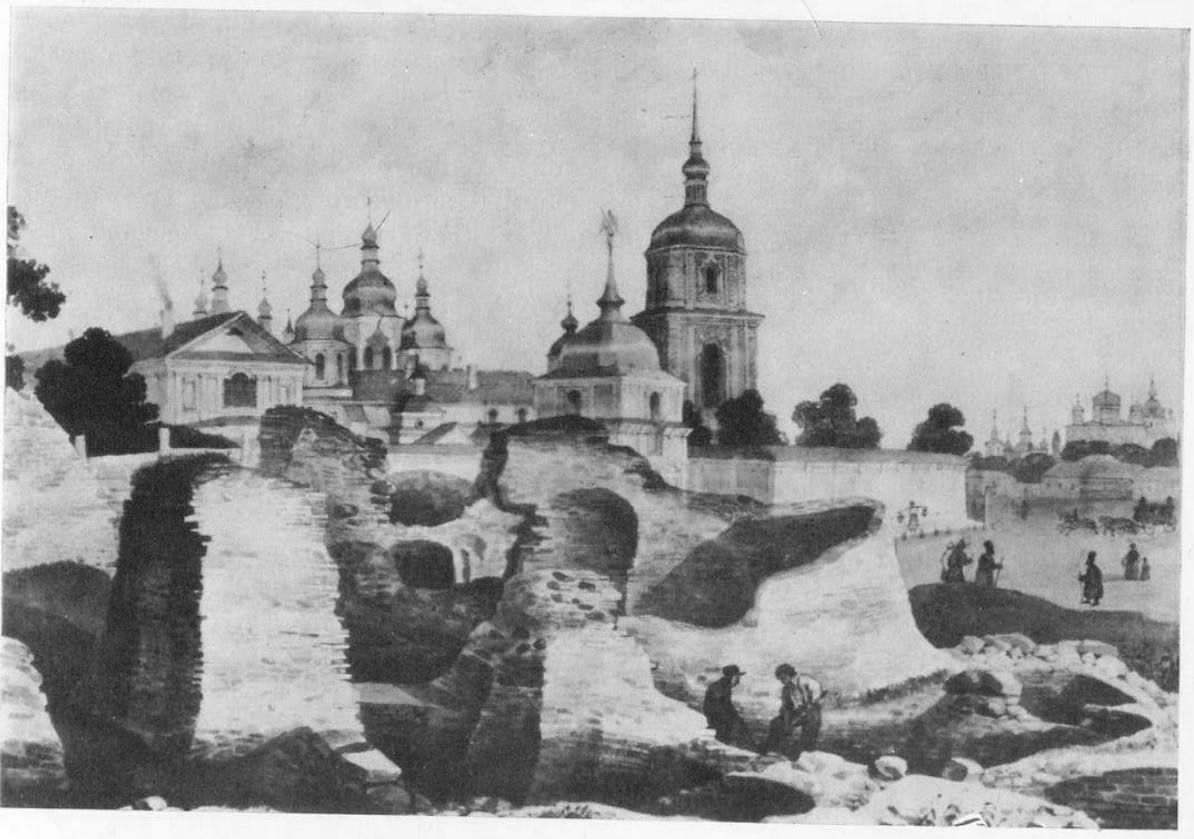
\includegraphics[width=\linewidth]{chast-volga/dir/irinsaj.jpg}

\textit{Развалины, рисунок М. Сажина, 1840-е.}
\end{center}


\begin{center}
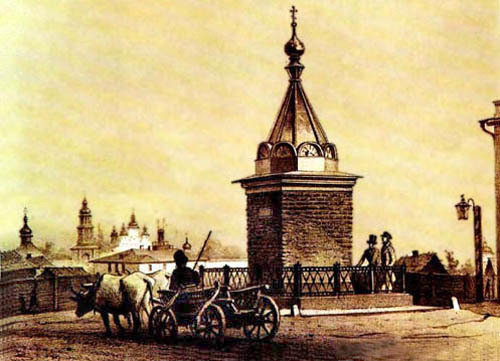
\includegraphics[width=\linewidth]{chast-volga/dir/irininsky_pamyatnik.jpg}

\textit{Дореволюционный памятник св. Ирины.}
\end{center}
\vspace*{\fill}
\newpage

В середине 19 века развалины «церкви святой Ирины» частью разобрали, частью засыпали, прокладывая Владимирскую улицу, а один столб от давнего здания оставили и, обложив кирпичом и увенчав крышей, превратили в памятник на углу Владимирской и Ирининской. Потому последняя и носит такое имя. Памятник снесли ночью с 26 на 27 марта 1932 года.

Лаврский архимандрит 17 века Иннокентий Гизель тоже считал, что церковь святой Ирины была «недалече от Святыя Софии». А Максим Берлинский думал, будто при Несторе существовала еще другая церковь Ирины, в ином месте, ибо нелогично хоронить Аскольда в одном месте, а Дира – много дальше.

Но современные историки приняли положение, что церковь святой Ирины находилась близ Софии, однако не определились, какие именно остались от нее развалины. То ли изученные Лохвицким в 19 веке, то ли Тимуром Бобровским в 21-м, в усадьбе заповедника Софии (эти же развалины в 1909 раскапывал Дмитрий Милеев)\footnote{Кстати, о ближайшей местности. П. Полевой во втором томе «Очерки русской истории в памятниках быта» пишет\cite[стр. 6]{polevoy01}:

\begin{quotation}
При земляных работах, предпринятых в 1874 году для расчистки места между улицами Прорезною и Фундуклиевскою, случайно наткнулись на обширное и весьма древнее кладбище. Судя по чрезвычайному множеству скелетов, которые уже и до этой находки в различное время были находимы около памятника, поставленнаго на месте бывшей церкви св. Ирины, а также близ Миниховского вала и на Елисаветинской улице – следует заметить, что кладбище это занимало весьма обширное пространство и много веков кряду служило местом погребения обширному и древнему поселению, находившемуся на месте нынешнего Киева.

Скелеты попадались большею частью на глубине 2 1/5 аршин, лежали, в большей части случаев, по направлению от севера к югу. При некоторых найдены были только кругловатые, просверленные посередине, камни, величиною в кулак; при многих – бусы из краснаго шифера, которыя, как мы уже знаем, в обилии производились в местности Овручского уезда, Волынской губернии, близ села Каменьшины. 

Среди могил попадались и такия, которыя вырыты были в роде небольших пещерок, и в них под низким сводом поставлены горшки с пеплом и обожженными костями. Свод и боковыя стенки таких могил были начисто вымазаны глиною, и глина эта обожжена. Кроме этого могил, среди того же кладбища попадались круглыя, глубокия ямы (12 фут. в поперечнике и 4 арш. глубины) с остатками очагов, сложенных из песчаника и других камней; они носили на себе явныя следы огня. 

Среди наполняющего эти ямы чернозема находили множество обугленных и раздробленных костей домашних животных (лошадей, рогатаго скота и свиней). Ясно, что эти очаги были также, вместе с кладбищем, остатками какого-то весьма древнего поселения, бывшаго на месте Киева в такую отдаленную эпоху, когда местное население еще не успело завести торговыя отношения с цивилизованными народами.
\end{quotation}}.

Где во времена Нестора была церковь святой Ирины, мне неясно, да и указание «за святой Ориной» мало что говорит. Сколь далеко «за»?

Как бы ни было, Олег с Игорем, убив Оскольда и Дира, похоронил их в курганах, память о которых сохранялась столетиями. Кем же были они, Оскольд и Дир – залётными властителями Киева, или законными правителями, намеренно, в летописи, лишенными принадлежности ко княжескому роду?

Здесь важно понятие родства и знатности. Рюрик и его братья – князья по происхождению, но мы помним, сколь много сомнений возникает при попытке углубить их родословную до Пруса. Вне этой, по сути, ныне голословной попытки, Рюрик возникает в истории из ниоткуда, из неведомых нам глубин истории. Это ниоткуда, возможно, появилось по злоумышлению противников рода Рюрика. Либо сами Рюриковичи решили нечто скрыть. Не разобрать.

Вещий Олег тоже приходит из пустоты, которую мы впрочем немного развеем далее. А по летописям у него в прошлом такая же тьма, как у Рюрика. Олег то племянник рюриков, то другой родственник – причем «рода княжего», то просто воевода.

С Аскольдом и Диром не легче. Один источник утверждает про Рюрика:

\begin{quotation}
Имея же у себе два воеводы асколд и дир, не его племени суща, ни княжеска, ни болярска.
\end{quotation}

Не племени Рюрика – значит, не родственники. И не княжеского рода, и не бояре. Так, военачальники. Хотя по известным спискам иначе: «не племени его, но боярина». Бояре, но всё равно чернь против знатного Игоря и Олега, который хоть и не наследник Рюрика, однако, по собственным олеговым словам, княжеского рода.

Основные летописи считают Аскольда и Дира таки Русами. О Русах пишет и Фотий. И если на Царьград при нем нападали именно Аскольд и Дир, то проступает многоуровневый план захвата Киева Олегом.

По совокупности противоречивых данных, закрывая глаза на одни и принимая за истину другие, полагаю следующее.

Олег обдуманно, пошагово строил новое государство, которое мы зовем Киевской Русью. Он стоял не просто рядом с Рюриком, Синеусом и Трувором, но «за» ними. Эти три брата – «призванные на княженье» знатные Варяги из народа Русь. В самом ли деле их призвали княжить народы Словен, Чуди, Мери, Кривичи и Весь, либо Олег руками Рюрика и братьев его взял власть силой – дело стороннее. В истории Рюрик и братья – законные князья государственного образования, названного по имени народа, пришедшего с Рюриком – Руси. Руси, что расширяла свои границы согласно новым завоеваниям.

И князья по двое, затем в одиночку сходят в могилу, владения их соединяются. По смерти Рюрика они достались бы наследнику – Игорю, но тот оказывается детеськ, и править всем приходится регенту Олегу. Пройдет много лет, Игорь станет здоровым дядькой, а Олег всё будет регенствовать.

Но вот Рюрик умер, и Олегу с Русами не сидится в стольном Новгороде. Надо расширять владения на полянские земли, брать Киев. А в Киеве пока свои, полянские правители. Олег не хочет от имени князя Игоря свергать другую законную власть, да еще портить отношения с Козарами (Хазарами), которым киевляне платят дань. Он посылает с этой целью Аскольда и Дира. Подстава!

Простаки, имея некоторое количество войска и ценные дары для Царьграда, метко «берут» Киев, да еще злят набегом Царьград.

Кто теперь Аскольд и Дир? Для новгородских Русов они – воры, присвоили дары, которые предназначались Царьграду. Для Полян-киевлян Аскольд и Дир – захватчики, сместившие местную власть. Для Византии – те же воры, да еще опасные соседи.

Пора действовать Вещему Олегу со знатным князем Игорем. Они приходят и уничтожают выскочек Аскольда и Дира.

Итоги блестящего выхода на сцену. Русы довольны – воры покараны. Киевляне освобождены от выскочек, да еще обретают знатного князя. Византия видит это и чувствует себя спокойно – злодеи повержены, а Киевом владеет отпрыск княжеского роду, архонт.

А если Аскольд с Диром еще и вывели Полян из-под дани Козарам, то пусть Козаре спросят с покойников, а не Игоря Рюриковича.

После захвата власти в Киеве, Олег строит в нем б\'ольший город, то бишь крепость, начинает тут княжить (а в Новгороде садит наместника), переносит столицу – стол, престол – в Киев.


% и говорит исторические слова: «се буди мти градом рускими». В иных списках это звучит так: «се буди мати всем градом Руским». Ученые трактуют слово «мати» как «мать» и начинают рассуждать, мол, город-то мужского рода, а почему же мать, а вот у скандинавов город рода женского, и потому...


%\begin{center}
%\includegraphics[width=\linewidth]{volga/IPAT-MTI.png}
%\end{center}


%\begin{center}
%\includegraphics[width=\linewidth]{volga/MTI-LAVR-STROKA.png}
%\end{center}


%А «мти» это вообще глагол. Если подразумевалось «мати»\footnote{В украинском языке сохранилось «мати» («маты») – «иметь».}, Олег употребил его в значении «иметь». Киев будет иметь все города Руские, то есть будет ими владеть, получать с них дань. Вот и всё.

%Киев-то теперь новая столица, не Новгород. Значит Киев, как стольный град Олега, будет теперь «мати», иметь остальные грады.

%Либо «мти» – слово того же корня, что «мыто». Значение особо не меняется. Киев будет мти, мытить, собирать мыто со всех городов русских, подвластных Руси. Это и есть назначение столицы, собирать налоги с других городов страны.

%Таково значение слов Олега.
